\newcommand{\figureADC}[1]{
  \def\lang{\detokenize{#1}}
  \def\langRu{\detokenize{ru}}
  \def\langEn{en}
  \def\figureCaption{XXX: No translation.}
  \ifx \lang\langRu
  \def\figureCaption{
    Схематическое изображение 10-битного аналогово-цифрового
    преобразователя (АЦП.)
  }
  \fi
  \if \lang\langEn
  \def\figureCaption{
    Schematic depiction of the 10-bit analog-to-digital converted (ADC.)
  }
  \fi
  \begin{figure}[ht]
    \centering
    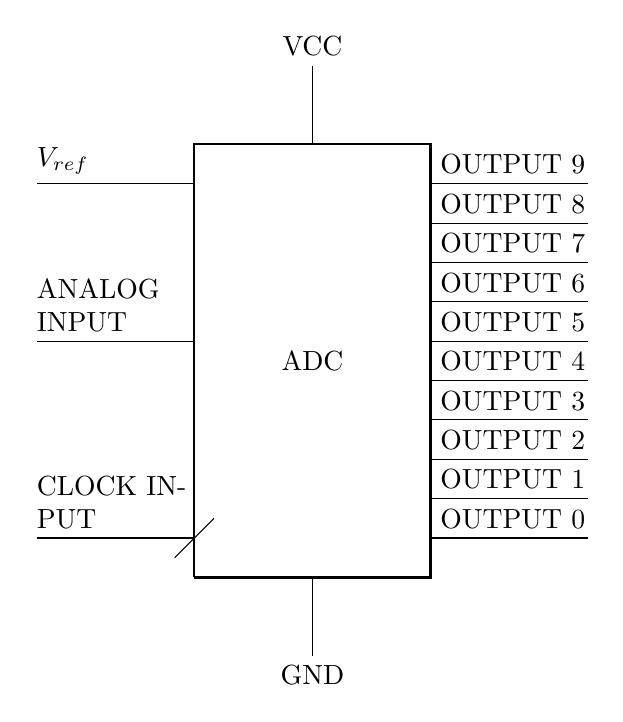
\begin{tikzpicture}
      \draw[thick] (0, 0) -- (0, 5.5) -- (3, 5.5) -- (3, 0) -- (0, 0);
      \draw (1.5, 2.5) node[right, above] {ADC};
      \draw (1.5, 5.5) -- (1.5, 6.5) node[right, above] {VCC};
      \draw (1.5, 0) -- (1.5, -1) node[right, below] {GND};
      \draw (-2, 5.0)
      -- (-1, 5.0) node[left, above, text width=2cm] {$V_{ref}$}
      -- (0, 5.0);
      \draw (0, 3.00)
      -- (-1, 3.00) node[left, above, text width=2cm] {ANALOG INPUT}
      -- (-2, 3.00);
      \draw (-2, 0.5)
      -- (-1, 0.5) node[left, above, text width=2cm] {CLOCK INPUT}
      -- (0, 0.5);
      \draw(-0.25, 0.25) -- (0.25, 0.75);
      \foreach \n/\y in {0/0.5, 1/1.0, 2/1.5, 3/2.0, 4/2.5, 5/3.0, 6/3.5, 7/4.0, 8/4.5, 9/5.0} {
        \draw (3, \y) node[anchor=south west] {OUTPUT \n} -- (5, \y);
      };
    \end{tikzpicture}
    \caption{\figureCaption}
    \label{fig:adc-schematics}
  \end{figure}
}
